\chapter{Arquitetura}

A arquitetura foi pensada para ser implementada com o Docker e Docker Compose. Cada
programa que precisa ser executado é rodado em um serviço separado. Exceto o Gunicorn,
todos os outros serviços usam imagens prontas do Docker Hub, o que oferece mais segurança
com as atualizações constantes.

\begin{figure}[ht]
    \begin{center}
    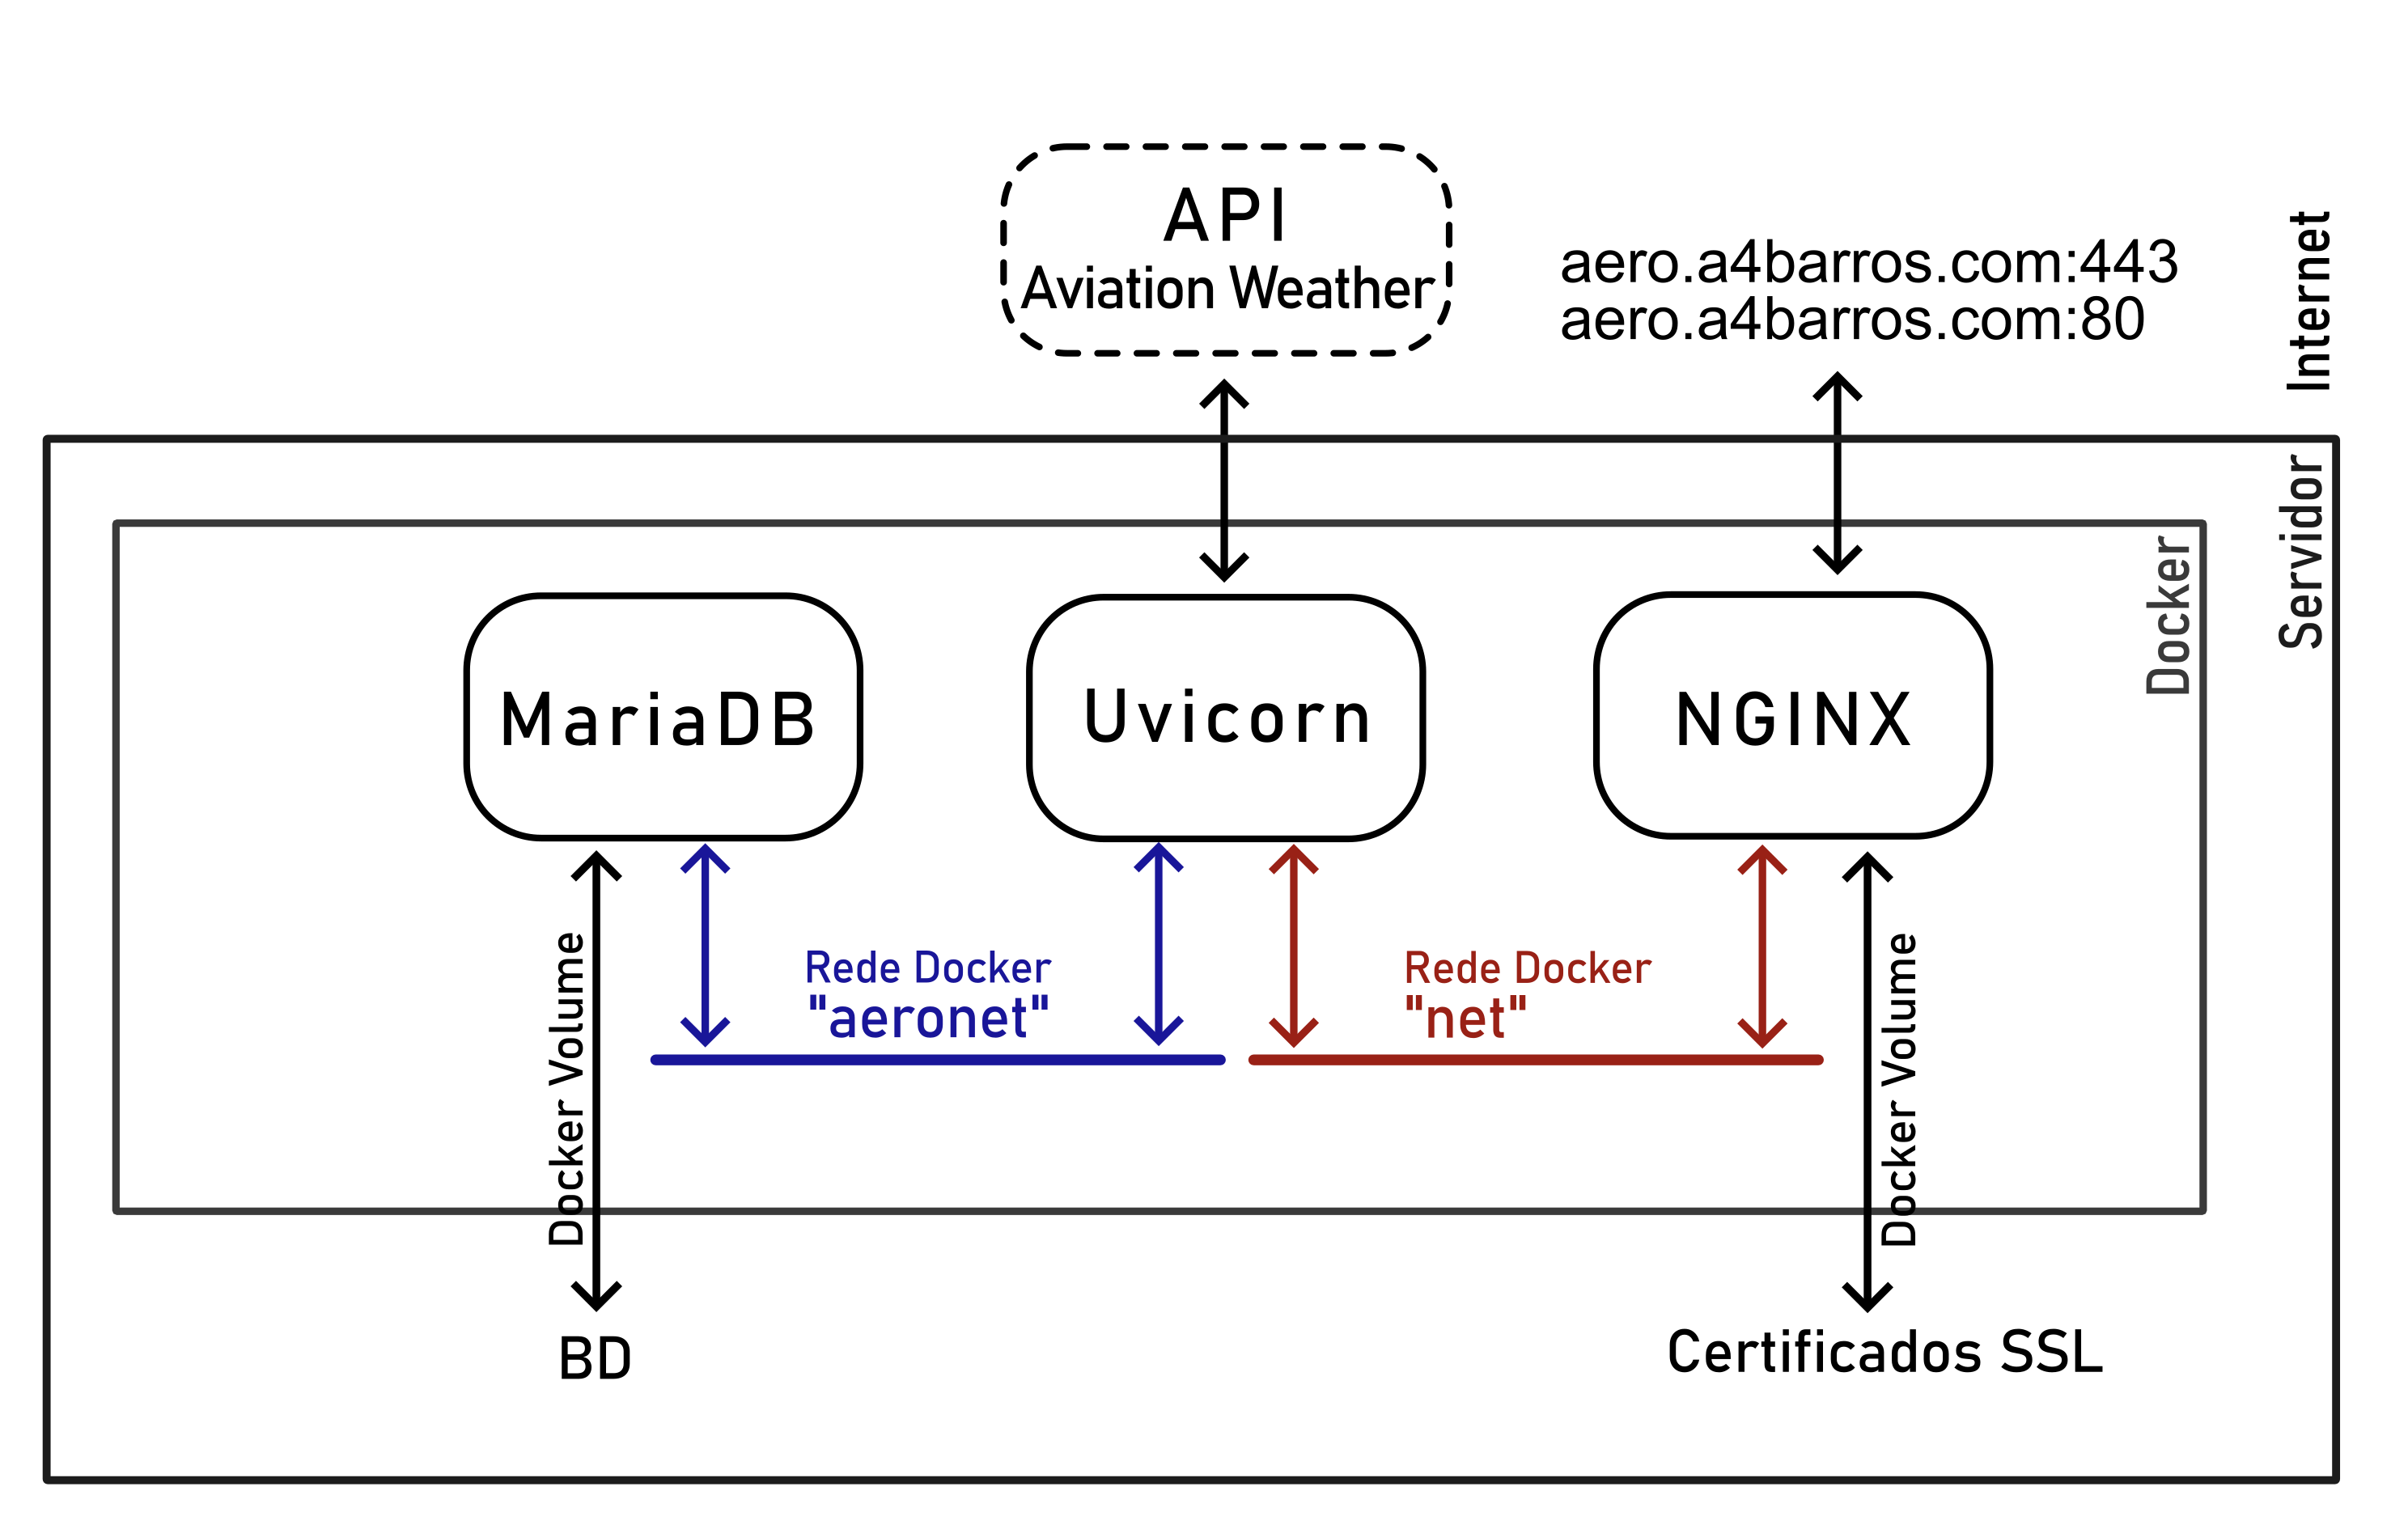
\includegraphics[width=\linewidth]{img/diagrama-arquitetura.png}
    \caption{Modelo de Arquitetura}
    \label{fig:arquitetura}
    \end{center}
\end{figure}

\section{Docker Network}
A porta 5000 do Gunicorn não estará disponível para todos os serviços. Por segurança, é usada a função de
"network". Observe no diagrama que a proxy NGINX compartilha com o Gunicorn a rede "net", para o NGINX,
o Gunicorn não pode ser acessado por \texttt{localhost:5000}, e sim por \texttt{http://aero:5000}, "aero"
sendo o nome do serviço no Docker Compose.


\section{Docker Secrets}

Para aumentar a segurança de acesso ao banco, é usada a funcionalidade "secrets". Nela, no Docker Compose,
você informa um arquivo de texto no host onde estará uma senha, uma senha por arquivo. No mesmo Compose,
você informa quais serviços têm acesso a cada senha. Caso o serviço de banco de dados, por exemplo, tenha
acesso a senha db-password.txt, será feito um bind do arquivo db-password.txt no host para o "/run/secret/db-password.txt"
no guest.
Tanto os bancos como o servidor Gunicorn usam este método para terem acesso às senhas dos bancos.

\section{Serviços}

\subsection{MariaDB}
Este banco de dados relacional guarda toda a informação mais ou menos fixa sobre os aeródromos,
conforme explicado no capítulo de modelo de dados.

\subsection{Proxy NGINX}
Faz o HTTPS funcionar, dá suporte ao HTTP/2 e ao header HTTP keep-alive. O Gunicorn só tem suporte
ao primeiro. De qualquer forma, a documentação do Gunicorn não recomenda que ele esteja diretamente
ligado à Internet \cite{nginx-gunicorn}. Já que tenho outros projetos na mesma máquina, uso subdomínios.
Na configuração do NGINX, o server block com hostname aero.a4barros.com é redirecionado para 
o endereço interno "https://aero:5000".

\section{Flask/Gunicorn}

Já que o Gunicorn é o serviço principal: o servidor onde o backend implementado em Flask roda,
fiz um Dockerfile próprio iniciando a partir de uma imagem do Alpine, devido a ser lightweight.
O Python e as dependências do projeto são instalados automaticamente pelo Dockerfile e, por
fim, o arquivo de entrada \texttt{server.py} é executado usando o servidor Gunicorn. As configurações
dele ficam no arquivo \texttt{gunicorn\_config.py} e apenas configura a porta para 5000 e usa três workers.

A documentação do Gunicorn informa a seguinte fórmula para determinar a quantidade de workers. \cite{number-work}

\begin{equation} 
    \begin{split}
        N_{worker} = 2 * N_{cores} + 1 \\
        N_{worker} = 2 * 1 + 1 = 3 
    \end{split}
\end{equation}

\section{Produção}
O site se encontra em produção no endereço https://aero.a4barros.com. Ele está hospedado em uma VPS
com as seguintes características:

\begin{itemize}
    \item \textbf{CPU:} AMD EPYC 7713 (1 core disponível) @ 2GHz
    \item \textbf{RAM:} 1GB
    \item \textbf{Armazenamento:} 25GB
    \item \textbf{SO:} Ubuntu 22.04.4 LTS
\end{itemize}

\begin{figure}[ht]
    \begin{center}
    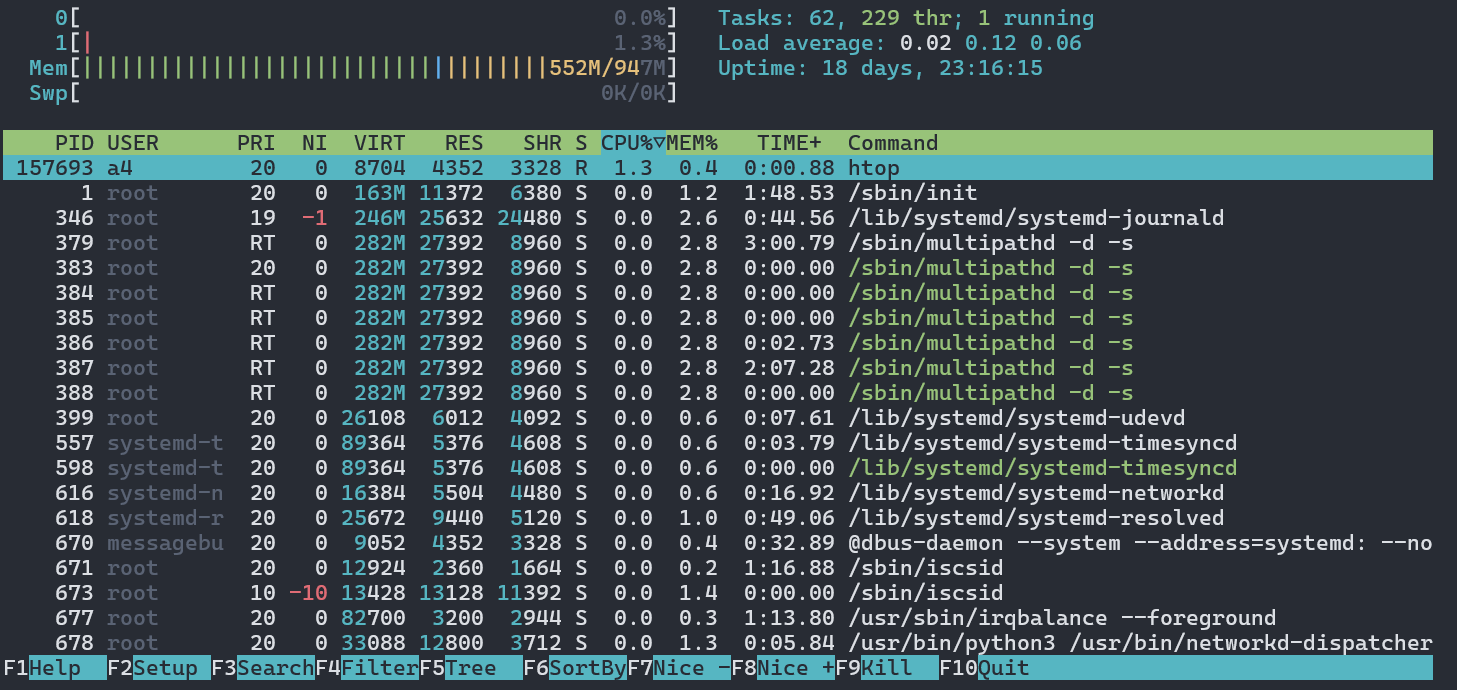
\includegraphics[width=400pt]{img/prod-idle.png}
    \caption{Uso do sistema em baixa demanda}
    \label{fig:prod-idle}
    \end{center}
\end{figure}

Mesmo com uma configuração bastante modesta, o sistema roda sete containers Docker, usando 
aproximadamente metade da memória primária (RAM) em idle.

\begin{figure}[ht]
    \begin{center}
    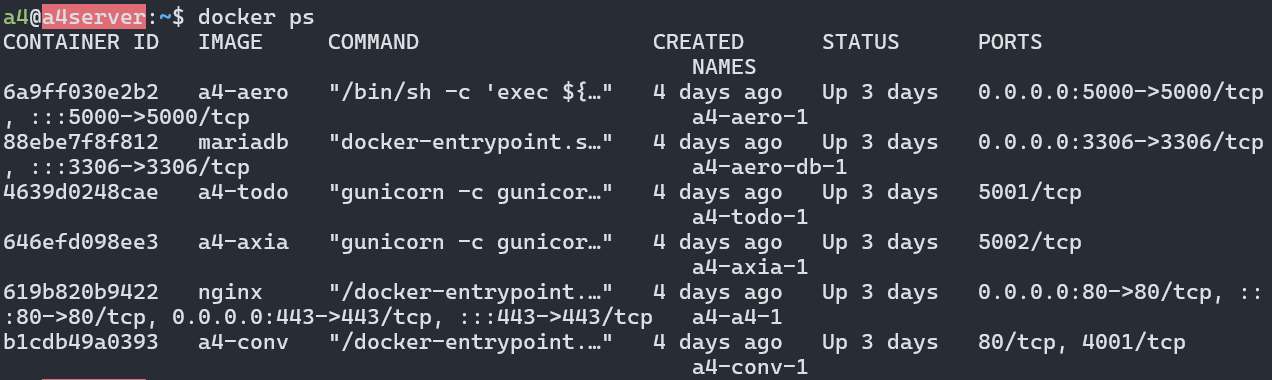
\includegraphics[width=400pt]{img/containers.png}
    \caption{Containers Docker em execução}
    \label{fig:containers}
    \end{center}
\end{figure}

\section{Diagrama de sequência}

\begin{figure}[ht]
    \begin{center}
    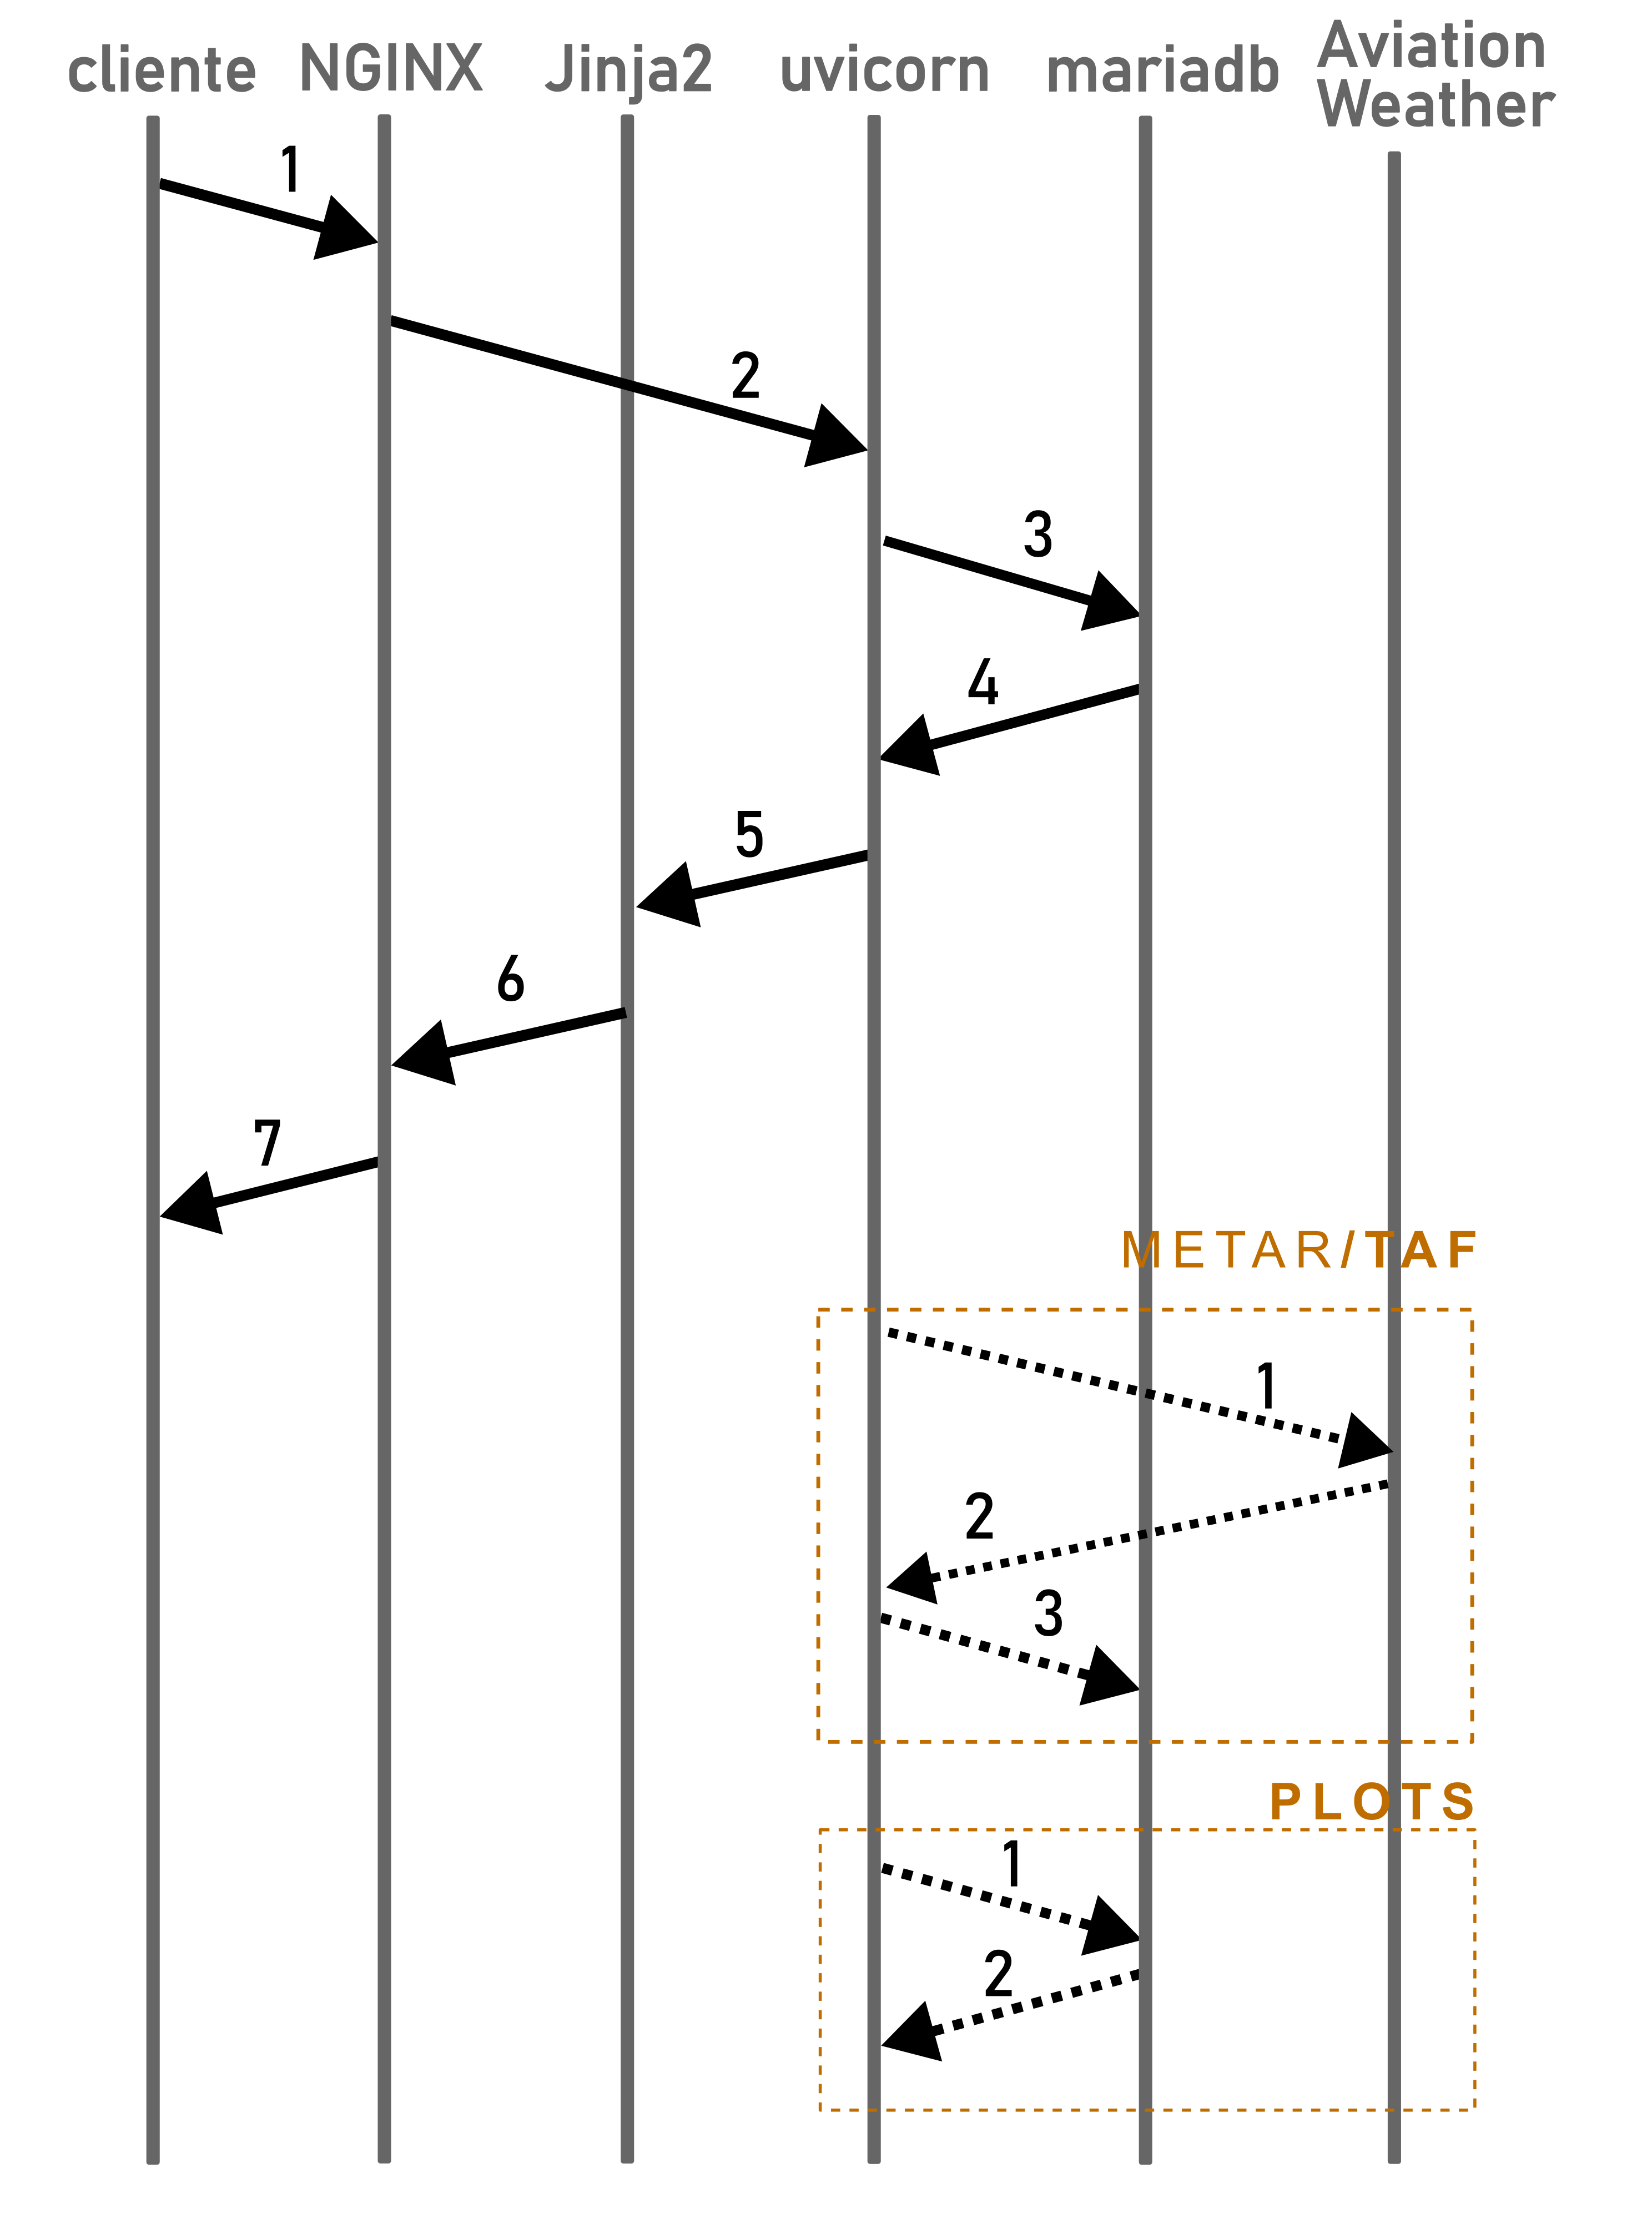
\includegraphics[width=0.5\linewidth]{img/diagrama-tempo.png}
    \caption{Diagrama de sequência}
    \label{fig:tempo}
    \end{center}
\end{figure}

\begin{enumerate}
\item O usuário realiza uma requisição para a rota raiz ou "/info/\{icao\}".
\item Um servidor NGINX funcionando como proxy realiza o limite de requisições por segundo
e bloqueia user-agents que aparentem ser robôs. Caso a requisição passe pelo filtro, é
realizado um proxy-pass para o servidor Gunicorn.
\item Para a rota raiz, é feito um SELECT no banco para pegar informações de todos os
aeroportos. Na rota "/info/\{icao\}", é feito um SELECT-WHERE para buscar apenas um aeroporto.
A ORM é usada para isto, portanto os comandos SQL não aparecem diretamente no código.
\item O banco de dados responde à requisição. Para a rota "/info/\{icao\}", é verificado 
se o METAR existente no banco é válido para aquela hora. Se for, o sistema vai para o passo 8;
se não, continua para o passo 5.
\item É feita uma requisição para a API do Aviation Weather pedindo o METAR para o 
aeroporto em questão. O sistema vai para o passo 3.
\item A API responde.
\item O METAR atualizado é gravado no banco.
\item O servidor envia as informações necessárias ao Jinja2 para a geração da página.
\item A página HTML é gerada.
\item O usuário recebe esta página.
\end{enumerate}
